
\begin{figure}[t]
\centering
\definecolor{openarm}{HTML}{2A78D6}
\definecolor{bndarm}{HTML}{C4551F}
\definecolor{brokerc}{HTML}{9A7A3E}
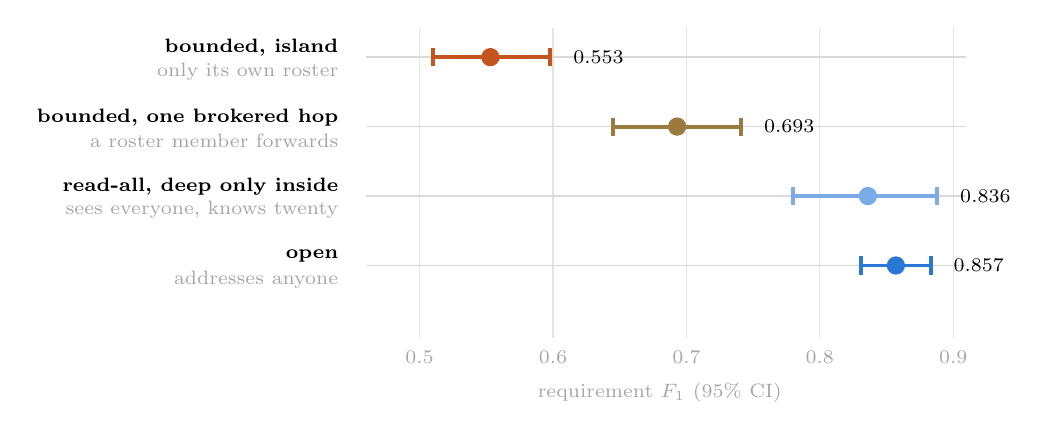
\begin{tikzpicture}[x=1.05cm,y=1.05cm,font=\small]
\draw[gray!22] (0.645,-0.30) -- (0.645,3.45);
\node[gray!70,font=\scriptsize,anchor=north] at (0.645,-0.34) {0.5};
\draw[gray!22] (2.259,-0.30) -- (2.259,3.45);
\node[gray!70,font=\scriptsize,anchor=north] at (2.259,-0.34) {0.6};
\draw[gray!22] (3.873,-0.30) -- (3.873,3.45);
\node[gray!70,font=\scriptsize,anchor=north] at (3.873,-0.34) {0.7};
\draw[gray!22] (5.486,-0.30) -- (5.486,3.45);
\node[gray!70,font=\scriptsize,anchor=north] at (5.486,-0.34) {0.8};
\draw[gray!22] (7.100,-0.30) -- (7.100,3.45);
\node[gray!70,font=\scriptsize,anchor=north] at (7.100,-0.34) {0.9};
\draw[gray!30,line width=.5pt] (0,3.10) -- (7.25,3.10);
\draw[bndarm,line width=1.4pt] (0.807,3.10) -- (2.227,3.10);
\draw[bndarm,line width=1.4pt] (0.807,2.99) -- (0.807,3.21);
\draw[bndarm,line width=1.4pt] (2.227,2.99) -- (2.227,3.21);
\filldraw[bndarm] (1.501,3.10) circle (3.1pt);
\node[font=\scriptsize,anchor=west] at (2.387,3.10) {0.553};
\node[font=\scriptsize\bfseries,anchor=east,align=right] at (-0.22,3.21) {bounded, island};
\node[font=\scriptsize,gray!70,anchor=east,align=right] at (-0.22,2.93) {only its own roster};
\draw[gray!30,line width=.5pt] (0,2.26) -- (7.25,2.26);
\draw[brokerc,line width=1.4pt] (2.985,2.26) -- (4.534,2.26);
\draw[brokerc,line width=1.4pt] (2.985,2.15) -- (2.985,2.37);
\draw[brokerc,line width=1.4pt] (4.534,2.15) -- (4.534,2.37);
\filldraw[brokerc] (3.760,2.26) circle (3.1pt);
\node[font=\scriptsize,anchor=west] at (4.694,2.26) {0.693};
\node[font=\scriptsize\bfseries,anchor=east,align=right] at (-0.22,2.37) {bounded, one brokered hop};
\node[font=\scriptsize,gray!70,anchor=east,align=right] at (-0.22,2.09) {a roster member forwards};
\draw[gray!30,line width=.5pt] (0,1.42) -- (7.25,1.42);
\draw[openarm!62,line width=1.4pt] (5.164,1.42) -- (6.906,1.42);
\draw[openarm!62,line width=1.4pt] (5.164,1.31) -- (5.164,1.53);
\draw[openarm!62,line width=1.4pt] (6.906,1.31) -- (6.906,1.53);
\filldraw[openarm!62] (6.067,1.42) circle (3.1pt);
\node[font=\scriptsize,anchor=west] at (7.066,1.42) {0.836};
\node[font=\scriptsize\bfseries,anchor=east,align=right] at (-0.22,1.53) {read-all, deep only inside};
\node[font=\scriptsize,gray!70,anchor=east,align=right] at (-0.22,1.25) {sees everyone, knows twenty};
\draw[gray!30,line width=.5pt] (0,0.58) -- (7.25,0.58);
\draw[openarm,line width=1.4pt] (5.987,0.58) -- (6.826,0.58);
\draw[openarm,line width=1.4pt] (5.987,0.47) -- (5.987,0.69);
\draw[openarm,line width=1.4pt] (6.826,0.47) -- (6.826,0.69);
\filldraw[openarm] (6.406,0.58) circle (3.1pt);
\node[font=\scriptsize,anchor=west] at (6.986,0.58) {0.857};
\node[font=\scriptsize\bfseries,anchor=east,align=right] at (-0.22,0.69) {open};
\node[font=\scriptsize,gray!70,anchor=east,align=right] at (-0.22,0.41) {addresses anyone};
\node[gray!70,font=\scriptsize,anchor=north] at (3.550,-0.72) {requirement $F_1$ (95\% CI)};
\end{tikzpicture}
\caption{An introduction does work an endorsement does not. All four rows are formation
manipulations, and every one of them moves; every \txt{attribute} manipulation---including
the ones asserting exactly the trust a broker would carry---is flat. One brokered hop
recovers $+0.140$ (CI $[+0.073, +0.204]$) of the $0.304$ gap and cuts fabrication from
$0.223$ to $0.057$ per task; letting a bounded arm read the whole directory while keeping
deep relationships inside the roster is indistinguishable from full openness ($+0.019$,
spans zero). Depth of relationship is not what is bought here---a second reachable source
is.}
\label{fig:ladder}
\end{figure}
